\documentclass[conference]{IEEEtran}

\usepackage[utf8]{inputenc}
\usepackage[T1]{fontenc}
\usepackage[spanish,es-tabla,es-nodecimaldot]{babel}
\usepackage{amsmath,amssymb}
\usepackage{graphicx}
\usepackage{booktabs}
\usepackage{multirow}
\usepackage{xcolor}
\usepackage{url}
\usepackage{cite}

% Las figuras se toman de results/ (generadas por el notebook). En Overleaf: subir los PNG a una carpeta figures/.
\graphicspath{{../results/}{figures/}}

% Marca visible para lo que falta llenar (borrar antes de entregar)
\newcommand{\pend}[1]{\textcolor{red}{\textbf{[PENDIENTE: #1]}}}

\begin{document}

\title{Comparación de DenseNet121, ResNet18 y ViT-B/16 para la clasificación multi-etiqueta de radiografías de tórax en NIH ChestX-ray14}

\author{\IEEEauthorblockN{Alfredo Gallegos}
\IEEEauthorblockA{\textit{Maestría --- Deep Learning, Proyecto Final}\\
Universidad Panamericana, Aguascalientes, México\\
alfredo.gallegos.mtr@gmail.com}}

\maketitle

\begin{abstract}
La interpretación automática de radiografías de tórax es una de las aplicaciones más estudiadas del aprendizaje profundo en imagen médica. En este trabajo se comparan tres arquitecturas preentrenadas en ImageNet ---dos redes convolucionales (DenseNet121 y ResNet18) y un Vision Transformer (ViT-B/16)--- en la clasificación multi-etiqueta de 14 hallazgos radiológicos del conjunto NIH ChestX-ray14, bajo un mismo protocolo experimental y un mismo presupuesto de entrenamiento: un subconjunto de 12{,}000 imágenes con partición por paciente, transferencia de aprendizaje con el backbone mayormente congelado y cinco épocas. Se evalúa el desempeño (AUROC por clase y promedio, F1 con umbral ajustado en validación, intervalos de confianza al 95\% por bootstrap y comparaciones pareadas), el costo computacional y la interpretabilidad (Grad-CAM y mapas de atención). ResNet18 obtuvo el mayor AUROC promedio (0.760; IC 95\%: 0.736--0.781), frente a 0.742 de DenseNet121 y 0.745 de ViT-B/16; solo la diferencia con DenseNet121 fue estadísticamente significativa. ViT-B/16 requirió 12 veces más parámetros que DenseNet121 y fue 13 veces más lento en inferencia que ResNet18 sin mejorar el desempeño, por lo que en este escenario las CNN ofrecen un mejor compromiso entre desempeño y costo.
\end{abstract}

\begin{IEEEkeywords}
radiografía de tórax, ChestX-ray14, clasificación multi-etiqueta, DenseNet, ResNet, Vision Transformer, transferencia de aprendizaje, Grad-CAM
\end{IEEEkeywords}

% =====================================================================
\section{Introducción}
% =====================================================================

La radiografía de tórax es el estudio de imagen más solicitado en la práctica clínica: es barata, rápida y de baja dosis, y es la primera herramienta para detectar condiciones como derrame pleural, neumonía, neumotórax o cardiomegalia. Su volumen, sin embargo, supera con frecuencia la capacidad de los radiólogos disponibles, y su lectura es difícil: los hallazgos se superponen en una proyección bidimensional, varios pueden coexistir en una misma imagen y algunos ---como los nódulos pequeños--- ocupan una fracción mínima del campo. Estas condiciones han motivado el uso de modelos de aprendizaje profundo como apoyo a la priorización y al diagnóstico.

La publicación del conjunto NIH ChestX-ray14~\cite{wang2017chestxray}, con más de cien mil radiografías etiquetadas con 14 hallazgos, convirtió a este problema en un banco de pruebas estándar. Sobre él, las redes neuronales convolucionales (CNN) ---en particular DenseNet121 en el trabajo CheXNet~\cite{rajpurkar2017chexnet}--- se establecieron como la referencia. Más recientemente, los Vision Transformers (ViT)~\cite{dosovitskiy2021vit}, que sustituyen las convoluciones por mecanismos de auto-atención sobre parches de la imagen, han igualado o superado a las CNN en visión natural, pero a costa de más parámetros y de una mayor dependencia de grandes volúmenes de datos de preentrenamiento. Si esa ventaja se traslada a la radiografía de tórax, con datos limitados y etiquetas ruidosas, no es evidente.

El objetivo de este trabajo es comparar, bajo un mismo protocolo experimental y un mismo presupuesto de cómputo, tres arquitecturas representativas: DenseNet121, ResNet18 y ViT-B/16. La comparación considera tres ejes: (i) desempeño de clasificación multi-etiqueta, con métricas apropiadas para clases fuertemente desbalanceadas e intervalos de confianza; (ii) costo computacional, y (iii) interpretabilidad de las predicciones mediante Grad-CAM~\cite{selvaraju2017gradcam} y mapas de atención~\cite{abnar2020rollout}.

Las contribuciones son: un protocolo reproducible con partición por paciente (que evita la fuga de información entre entrenamiento y prueba); una evaluación que reporta AUROC por clase, F1 con umbrales elegidos en validación y comparaciones estadísticas pareadas entre modelos, y un análisis crítico del compromiso entre desempeño, costo e interpretabilidad de CNN y Transformers en este dominio.

% =====================================================================
\section{Estado del arte}
% =====================================================================

\subsection{Conjuntos de datos de radiografía de tórax}
Wang et~al.~\cite{wang2017chestxray} publicaron ChestX-ray8, posteriormente ampliado a ChestX-ray14: 112{,}120 radiografías frontales de 30{,}805 pacientes, con 14 etiquetas de hallazgos extraídas automáticamente de los reportes radiológicos mediante procesamiento de lenguaje natural. Este etiquetado automático permitió construir un conjunto a gran escala, pero introduce ruido: Oakden-Rayner~\cite{oakdenrayner2020exploring} documentó discrepancias importantes entre las etiquetas y la revisión visual de las imágenes. Conjuntos posteriores como CheXpert~\cite{irvin2019chexpert} incorporaron etiquetas de incertidumbre y conjuntos de prueba anotados por radiólogos.

\subsection{Redes convolucionales}
ResNet~\cite{he2016resnet} introdujo las conexiones residuales, que permiten entrenar redes muy profundas al facilitar el flujo del gradiente. DenseNet~\cite{huang2017densenet} lleva esta idea más lejos: cada capa de un bloque recibe como entrada la concatenación de los mapas de todas las capas anteriores, lo que reutiliza características y reduce el número de parámetros. CheXNet~\cite{rajpurkar2017chexnet} afinó una DenseNet121 preentrenada en ImageNet~\cite{deng2009imagenet} sobre ChestX-ray14 completo, reportando un AUROC promedio cercano a 0.84 en los 14 hallazgos y un desempeño comparable al de radiólogos en la detección de neumonía, y se convirtió en la referencia para este conjunto.

\subsection{Transformers en visión}
El Transformer~\cite{vaswani2017attention} se basa por completo en auto-atención. El Vision Transformer (ViT)~\cite{dosovitskiy2021vit} lo aplica a imágenes dividiéndolas en parches de $16\times16$ píxeles, que se proyectan linealmente como tokens junto con un token de clase \texttt{[CLS]}. Al carecer de los sesgos inductivos de las convoluciones (localidad y equivarianza a traslaciones), el ViT requiere preentrenamiento a gran escala para superar a las CNN, pero a cambio modela relaciones globales desde las primeras capas. Raghu et~al.~\cite{raghu2021vit} mostraron que las representaciones de los ViT difieren cualitativamente de las de las CNN, con mayor uso de información global. En radiografía de tórax, Murphy et~al.~\cite{murphy2022vit} compararon Transformers (DeiT) con CNN como DenseNet121, ambos preentrenados en ImageNet, sobre ChestX-ray14 y MURA: los Transformers obtuvieron AUROC ligeramente menores ---diferencias que los autores consideran probablemente despreciables en la práctica clínica--- y una eficiencia de muestra similar a la de DenseNet121. Más recientemente, Yanar et~al.~\cite{yanar2025mamba} evaluaron 14 arquitecturas CNN, Transformer y Mamba en ChestX-ray14 bajo condiciones de entrenamiento idénticas; los mejores resultados correspondieron a modelos híbridos Transformer--CNN (ConvFormer, con AUROC promedio de 0.841), seguidos de cerca por la CNN EfficientNet.

\subsection{Interpretabilidad}
Grad-CAM~\cite{selvaraju2017gradcam} genera mapas de activación ponderando los mapas de características de una capa convolucional por el gradiente de la clase objetivo. En Transformers, los pesos de atención ofrecen una explicación natural, aunque la atención de una sola capa puede ser engañosa; el \emph{attention rollout}~\cite{abnar2020rollout} combina la atención de todas las capas teniendo en cuenta las conexiones residuales. En imagen médica, estas herramientas son especialmente relevantes porque los modelos pueden aprender atajos (\emph{shortcuts}) ---marcas del hospital, texto o dispositivos--- en lugar de los signos clínicos~\cite{zech2018variable,degrave2021shortcuts}.

% =====================================================================
\section{Metodología}
% =====================================================================

\subsection{Datos y partición}
Se usó la distribución pública del conjunto en Kaggle~\cite{kaggle2018nih}, que incluye las imágenes y el archivo de etiquetas \texttt{Data\_Entry\_2017.csv}. De sus 112{,}120 imágenes se muestrearon al azar 12{,}000 (semilla fija), un tamaño elegido por el presupuesto de cómputo y tiempo del proyecto. Cada imagen se representa con un vector binario $\mathbf{y}\in\{0,1\}^{14}$; la etiqueta ``No Finding'' corresponde al vector nulo, y una imagen puede tener varios hallazgos simultáneos. La partición en entrenamiento, validación y prueba (70/15/15\% de las imágenes) se realizó \textbf{por paciente}: los pacientes se asignaron aleatoriamente a un solo subconjunto, de modo que ningún paciente aparece en más de uno. Esto evita que el modelo se evalúe sobre pacientes ya vistos durante el entrenamiento, lo que inflaría las métricas. La Tabla~\ref{tab:datos} resume la partición; la prevalencia de cada hallazgo va del 0.18\% (Hernia) al 17.7\% (Infiltration).

\begin{table}[t]
\centering
\caption{Partición por paciente y positivos por clase.}
\label{tab:datos}
\begin{tabular}{lrrr}
\toprule
 & Entrenamiento & Validación & Prueba \\
\midrule
Imágenes & 8{,}400 & 1{,}798 & 1{,}802 \\
Pacientes & 5{,}317 & 1{,}079 & 1{,}166 \\
\midrule
Atelectasis & 816 & 187 & 181 \\
Cardiomegaly & 205 & 53 & 42 \\
Effusion & 998 & 230 & 209 \\
Infiltration & 1{,}458 & 344 & 324 \\
Mass & 442 & 98 & 94 \\
Nodule & 467 & 113 & 95 \\
Pneumonia & 118 & 24 & 15 \\
Pneumothorax & 389 & 77 & 84 \\
Consolidation & 314 & 83 & 54 \\
Edema & 157 & 45 & 35 \\
Emphysema & 188 & 49 & 26 \\
Fibrosis & 127 & 21 & 33 \\
Pleural\_Thickening & 237 & 48 & 51 \\
Hernia & 12 & 1 & 8 \\
\bottomrule
\end{tabular}
\end{table}

\subsection{Preprocesamiento}
Las radiografías originales ($1024\times1024$, escala de grises) se redimensionan a $224\times224$, se replican en tres canales y se normalizan con la media y desviación estándar de ImageNet. Como aumento de datos se usa únicamente el volteo horizontal aleatorio en entrenamiento.

\subsection{Modelos}
Se usaron las implementaciones de \texttt{torchvision} con pesos preentrenados en ImageNet-1k: DenseNet121~\cite{huang2017densenet}, ResNet18~\cite{he2016resnet} y ViT-B/16~\cite{dosovitskiy2021vit} (12 bloques, 12 cabezas de atención, dimensión 768, 196 parches más el token \texttt{[CLS]}). En los tres se reemplazó la capa de clasificación por una capa lineal de 14 salidas y se congeló el backbone salvo su último bloque: el cuarto bloque denso y la normalización final en DenseNet121, el bloque \texttt{layer4} en ResNet18 y el último bloque del encoder en ViT-B/16. La Tabla~\ref{tab:params} resume el número de parámetros.

\begin{table}[t]
\centering
\caption{Parámetros de los modelos (millones).}
\label{tab:params}
\begin{tabular}{lrr}
\toprule
Modelo & Totales & Entrenables \\
\midrule
DenseNet121 & 6.97 & 2.17 \\
ResNet18 & 11.18 & 8.40 \\
ViT-B/16 & 85.81 & 7.10 \\
\bottomrule
\end{tabular}
\end{table}

\subsection{Entrenamiento}
Los tres modelos se entrenaron con el mismo protocolo: pérdida de entropía cruzada binaria sobre las 14 salidas,
\begin{equation}
\mathcal{L} = -\frac{1}{14}\sum_{c=1}^{14}\left[y_c\log\sigma(z_c) + (1-y_c)\log\left(1-\sigma(z_c)\right)\right],
\end{equation}
donde $z_c$ es el logit de la clase $c$ y $\sigma$ la función sigmoide; optimizador Adam~\cite{kingma2015adam} con tasa de aprendizaje $10^{-4}$, lotes de 32 imágenes y 5 épocas. Al final del entrenamiento se restauran los pesos de la época con menor pérdida de validación. Todos los experimentos usan la misma semilla y la misma partición. Se implementaron en PyTorch~\cite{paszke2019pytorch} y se ejecutaron en una GPU AMD Radeon RX 6800 XT (16\,GB) mediante ROCm.

\subsection{Evaluación}
La métrica principal es el área bajo la curva ROC (AUROC) por clase y su promedio sobre las 14 clases, que no depende de un umbral de decisión y es la métrica estándar en este conjunto~\cite{wang2017chestxray,rajpurkar2017chexnet}. Dado que la prevalencia de cada hallazgo va de menos del 1\% a cerca del 18\%, un umbral fijo de 0.5 produce muy pocas predicciones positivas; por ello, el umbral de cada clase se elige maximizando su F1 en el conjunto de \textbf{validación} y se aplica sin cambios al conjunto de prueba, donde se reportan F1 macro y micro. La exactitud por etiqueta se reporta solo como referencia, junto a la de un clasificador trivial que predice siempre ``sin hallazgo''.

Para cuantificar la incertidumbre se calcularon intervalos de confianza al 95\% mediante bootstrap~\cite{efron1993bootstrap} con 1000 remuestreos del conjunto de prueba. Los mismos remuestreos se aplicaron a los tres modelos, lo que permite comparaciones pareadas: la diferencia entre dos modelos se considera significativa si su intervalo de confianza no incluye el cero.

El costo computacional se midió como número de parámetros, tiempo promedio por época (entrenamiento más validación), memoria pico de GPU durante el entrenamiento y velocidad de inferencia (imágenes por segundo, lotes de 32 ya cargados en la GPU). Antes de medir se realizó un paso de calentamiento, y cada modelo se retiró de la GPU al terminar para que la memoria medida corresponda únicamente al modelo en curso.

\subsection{Interpretabilidad}
Para las CNN se usó Grad-CAM~\cite{selvaraju2017gradcam} sobre la última capa convolucional, tomando como objetivo la clase real de la imagen. Dados los mapas de características $A^k$ y el logit $y^c$, el mapa es
\begin{equation}
L^c = \mathrm{ReLU}\Big(\sum_k \alpha_k^c A^k\Big), \qquad \alpha_k^c = \frac{1}{Z}\sum_{i,j}\frac{\partial y^c}{\partial A^k_{ij}}.
\end{equation}
Para el ViT se visualizan la atención del token \texttt{[CLS]} hacia los parches en el último bloque y el \emph{attention rollout}~\cite{abnar2020rollout}: con $A_l$ la atención promedio de las cabezas en el bloque $l$, se define $\tilde{A}_l = \tfrac{1}{2}A_l + \tfrac{1}{2}I$ normalizada por filas, y $R = \tilde{A}_{12}\cdots\tilde{A}_{1}$; la fila de \texttt{[CLS]} de $R$ da la relevancia de cada parche. Ambos mapas del ViT son independientes de la clase.

% =====================================================================
\section{Resultados}
% =====================================================================

\subsection{Desempeño de clasificación}
La Tabla~\ref{tab:resultados} resume el desempeño en el conjunto de prueba (1{,}802 imágenes de 1{,}166 pacientes). ResNet18 obtuvo el mayor AUROC promedio (0.760), seguido de ViT-B/16 (0.745) y DenseNet121 (0.742). Las diferencias son pequeñas y sus intervalos de confianza se traslapan. En la comparación pareada, solo la ventaja de ResNet18 sobre DenseNet121 es significativa, tanto en AUROC ($+0.018$; IC 95\%: 0.001--0.035) como en F1 micro ($+0.016$; IC 95\%: 0.001--0.029). Entre ResNet18 y ViT-B/16 ($+0.015$ en AUROC; IC 95\%: $-0.004$--0.035) y entre ViT-B/16 y DenseNet121 ($+0.003$) no hay diferencias significativas, y el F1 macro es prácticamente idéntico en los tres (0.185--0.186).

La exactitud por etiqueta de los tres modelos (0.950) es igual a la del clasificador trivial que nunca predice un hallazgo (0.950), lo que confirma que no es una métrica informativa en este problema. Del mismo modo, con un umbral fijo de 0.5 el F1 macro es de apenas 0.012--0.037; al elegir el umbral de cada clase en validación sube a 0.185--0.186.

\begin{table*}[t]
\centering
\caption{Desempeño en el conjunto de prueba (IC al 95\% por bootstrap entre corchetes). F1 con umbral por clase elegido en validación.}
\label{tab:resultados}
\begin{tabular}{lccccc}
\toprule
Modelo & AUROC macro & F1 macro & F1 micro & F1 macro @0.5 & Mejor época \\
\midrule
DenseNet121 & 0.742 [0.717, 0.767] & 0.185 [0.168, 0.201] & 0.248 [0.231, 0.266] & 0.012 & 2 \\
ResNet18 & \textbf{0.760} [0.736, 0.781] & 0.186 [0.165, 0.204] & \textbf{0.264} [0.245, 0.283] & 0.037 & 2 \\
ViT-B/16 & 0.745 [0.718, 0.769] & 0.186 [0.166, 0.204] & 0.249 [0.232, 0.265] & 0.016 & 3 \\
\bottomrule
\end{tabular}
\end{table*}

La Fig.~\ref{fig:auroc} y la Tabla~\ref{tab:auroc} muestran el AUROC por clase. La variación entre hallazgos es mucho mayor que entre modelos: Emphysema, Edema y Effusion superan 0.82 en los tres modelos, mientras que Nodule, Infiltration y Pneumonia quedan por debajo de 0.69. La mayor diferencia entre arquitecturas aparece en Cardiomegaly (0.663 en DenseNet121 frente a 0.775 en ResNet18). Las clases con pocos positivos en prueba, como Hernia ($n=8$) y Pneumonia ($n=15$), tienen estimaciones inestables.

\begin{table}[t]
\centering
\caption{AUROC por clase en prueba ($n$ = positivos en prueba).}
\label{tab:auroc}
\begin{tabular}{lrccc}
\toprule
Hallazgo & $n$ & DenseNet & ResNet & ViT \\
\midrule
Emphysema & 26 & 0.880 & \textbf{0.890} & 0.864 \\
Edema & 35 & 0.851 & \textbf{0.872} & 0.841 \\
Effusion & 209 & 0.823 & \textbf{0.831} & 0.828 \\
Pneumothorax & 84 & 0.765 & \textbf{0.798} & 0.769 \\
Fibrosis & 33 & 0.771 & \textbf{0.782} & 0.755 \\
Atelectasis & 181 & 0.751 & \textbf{0.766} & 0.756 \\
Consolidation & 54 & 0.749 & \textbf{0.765} & 0.729 \\
Hernia & 8 & 0.722 & 0.728 & \textbf{0.780} \\
Mass & 94 & 0.736 & \textbf{0.759} & 0.728 \\
Pleural\_Thickening & 51 & \textbf{0.747} & 0.720 & 0.730 \\
Cardiomegaly & 42 & 0.663 & \textbf{0.775} & 0.751 \\
Infiltration & 324 & 0.657 & 0.661 & \textbf{0.680} \\
Nodule & 95 & \textbf{0.656} & 0.635 & 0.651 \\
Pneumonia & 15 & 0.612 & \textbf{0.652} & 0.563 \\
\bottomrule
\end{tabular}
\end{table}

\begin{figure}[t]
\centering
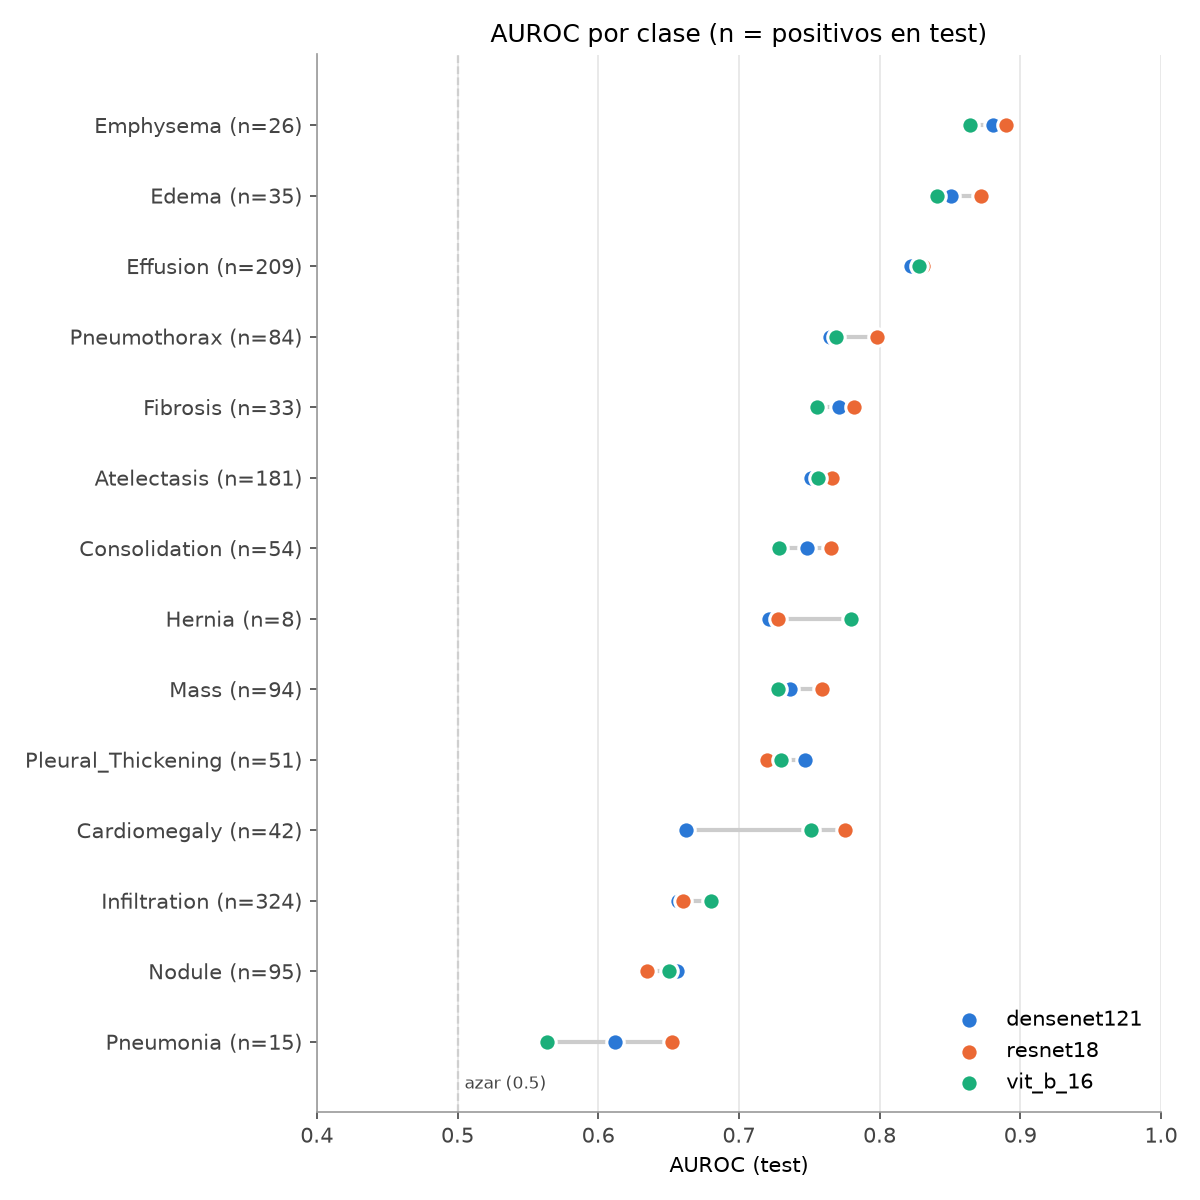
\includegraphics[width=\columnwidth]{auroc_per_class.png}
\caption{AUROC por clase en el conjunto de prueba ($n$ = positivos en prueba). La línea discontinua indica el desempeño aleatorio.}
\label{fig:auroc}
\end{figure}

\subsection{Convergencia}
La Fig.~\ref{fig:curvas} muestra la pérdida de validación por época. DenseNet121 y ResNet18 alcanzan su mínimo en la época 2 y ViT-B/16 en la época 3. ResNet18, el modelo con más parámetros entrenables (8.4M), se sobreajusta claramente a partir de la época 3: su pérdida de entrenamiento cae de 0.153 a 0.084 mientras la de validación sube de 0.173 a 0.203. DenseNet121 y ViT-B/16 se mantienen estables, con un aumento leve de la pérdida de validación al final.

\begin{figure}[t]
\centering
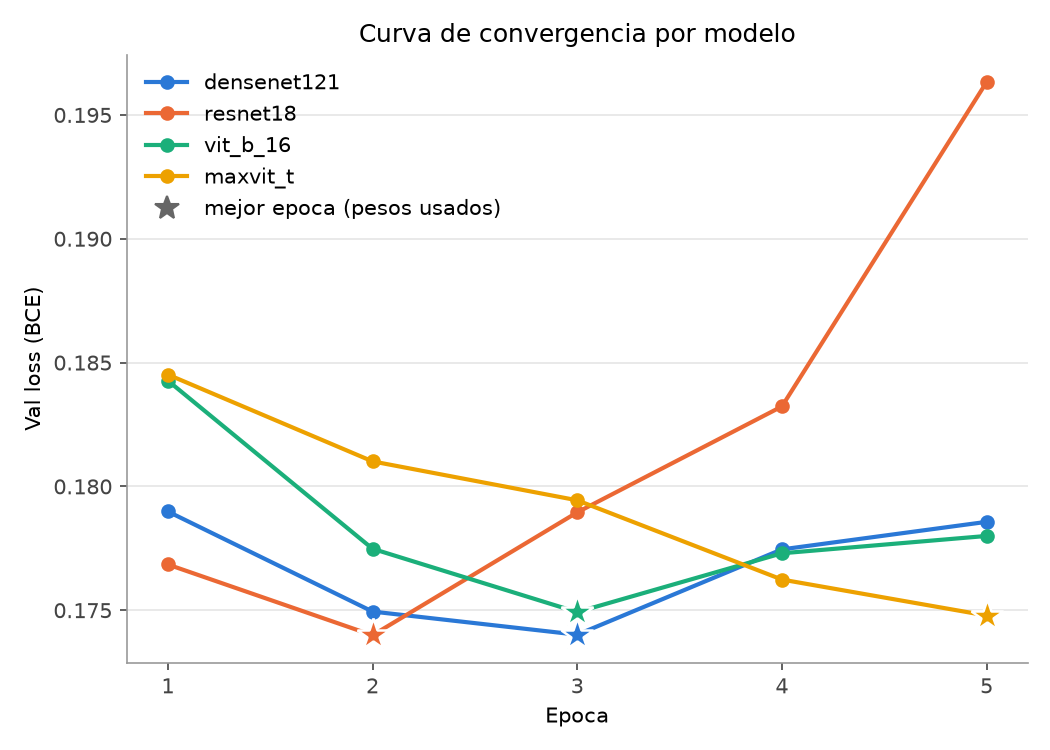
\includegraphics[width=0.9\columnwidth]{val_loss_curves.png}
\caption{Pérdida de validación por época. La estrella marca la época cuyos pesos se usan en la evaluación.}
\label{fig:curvas}
\end{figure}

\subsection{Costo computacional}
La Tabla~\ref{tab:costo} y la Fig.~\ref{fig:costo} resumen el costo. ViT-B/16 tiene 12.3 veces los parámetros de DenseNet121, usa 2.3 veces la memoria de GPU de ResNet18 durante el entrenamiento y procesa 359 imágenes por segundo en inferencia, frente a 4{,}653 de ResNet18 (13 veces más) y 1{,}145 de DenseNet121. El tiempo por época es más parecido entre modelos porque en las CNN lo domina la lectura y decodificación de las imágenes de $1024\times1024$, no el cómputo en la GPU.

\begin{table}[t]
\centering
\caption{Costo computacional (lotes de 32, $224\times224$).}
\label{tab:costo}
\begin{tabular}{lrrr}
\toprule
Modelo & s/época & Memoria (MB) & Inferencia (img/s) \\
\midrule
DenseNet121 & 41.3 & 442 & 1{,}145 \\
ResNet18 & 44.3 & 418 & 4{,}653 \\
ViT-B/16 & 57.8 & 980 & 359 \\
\bottomrule
\end{tabular}
\end{table}

\begin{figure*}[t]
\centering
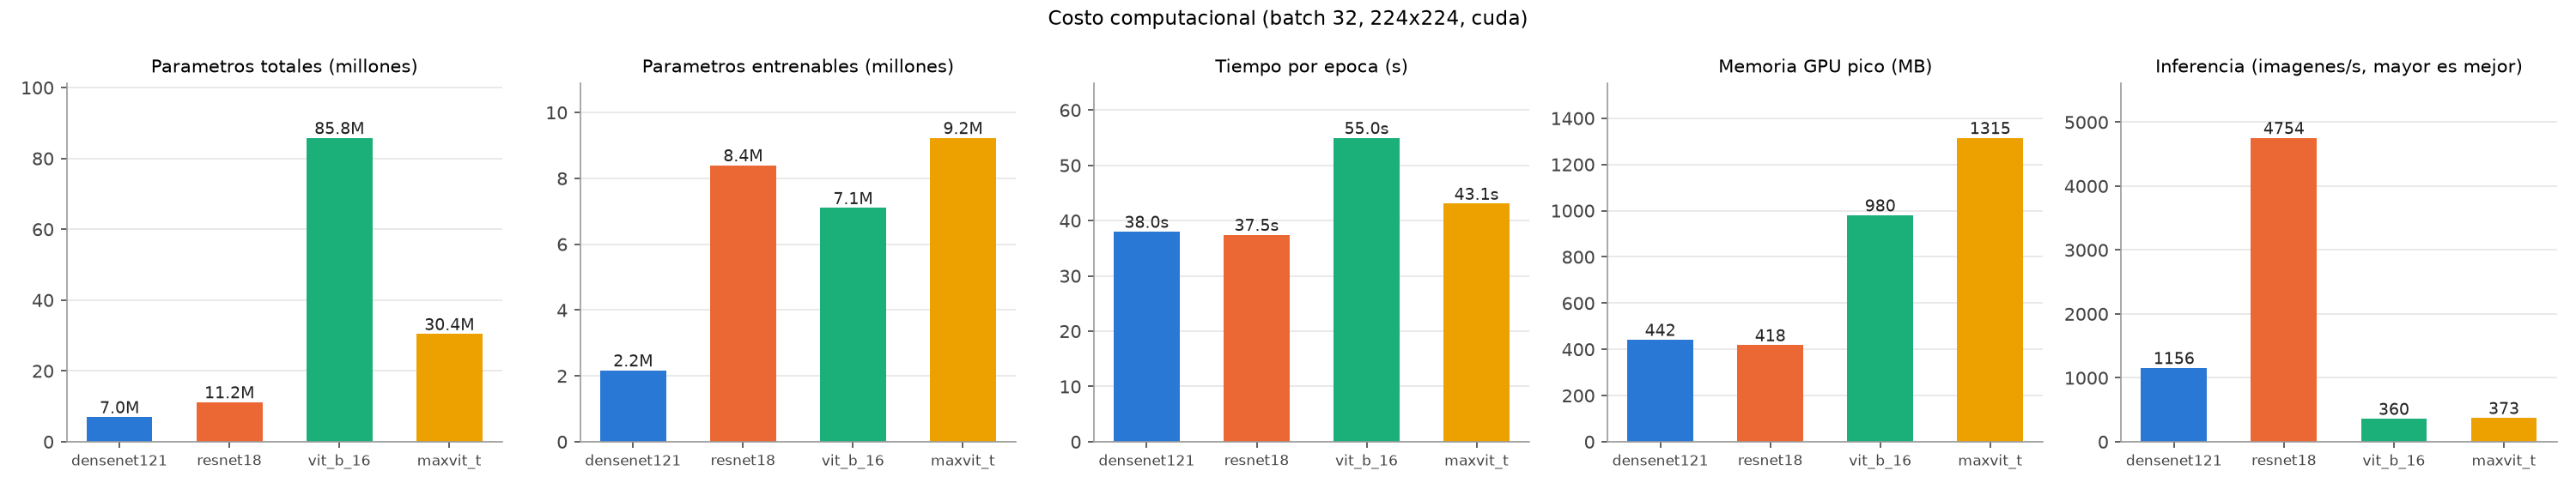
\includegraphics[width=\textwidth]{cost_comparison.png}
\caption{Costo computacional por modelo: parámetros totales y entrenables, tiempo por época, memoria pico de GPU y velocidad de inferencia.}
\label{fig:costo}
\end{figure*}

\subsection{Interpretabilidad}
Las Figs.~\ref{fig:gradcam} y~\ref{fig:atencion} muestran tres imágenes de prueba con un solo hallazgo. En el caso de Effusion, ambas CNN asignan una probabilidad alta (0.71 y 0.88) y concentran el Grad-CAM en la región torácica inferior, compatible con el hallazgo. En el caso de Infiltration, en cambio, los mapas se concentran en el borde superior de la imagen ---donde aparece la marca de texto ``PORTABLE''--- y fuera de los campos pulmonares, un patrón compatible con el aprendizaje de atajos descrito en la literatura~\cite{zech2018variable,degrave2021shortcuts}. En el caso de Atelectasis, con probabilidades de 0.04, el mapa de ResNet18 queda vacío. Para ViT-B/16, la atención del último bloque en el caso de Infiltration sí recorre ambos campos pulmonares, mientras que el rollout concentra buena parte de la relevancia en las esquinas de la imagen, un artefacto conocido de los mapas de atención que obliga a interpretarlos con cautela.

\begin{figure}[t]
\centering
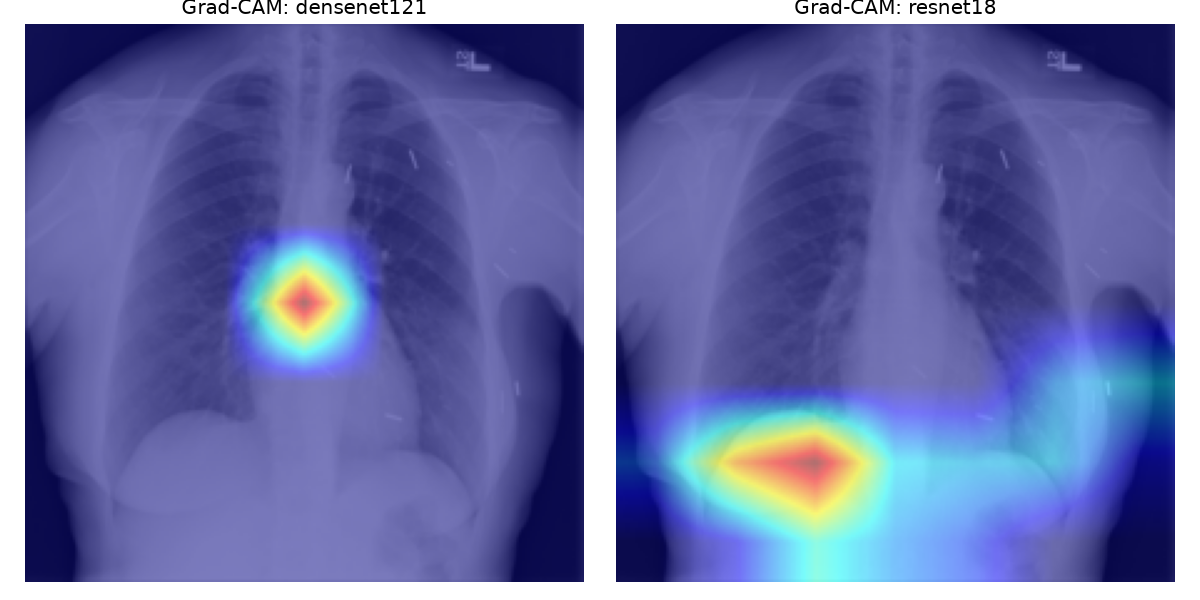
\includegraphics[width=\columnwidth]{gradcam_examples.png}
\caption{Grad-CAM de DenseNet121 y ResNet18 para la clase real de cada imagen, con la probabilidad asignada por cada modelo.}
\label{fig:gradcam}
\end{figure}

\begin{figure}[t]
\centering
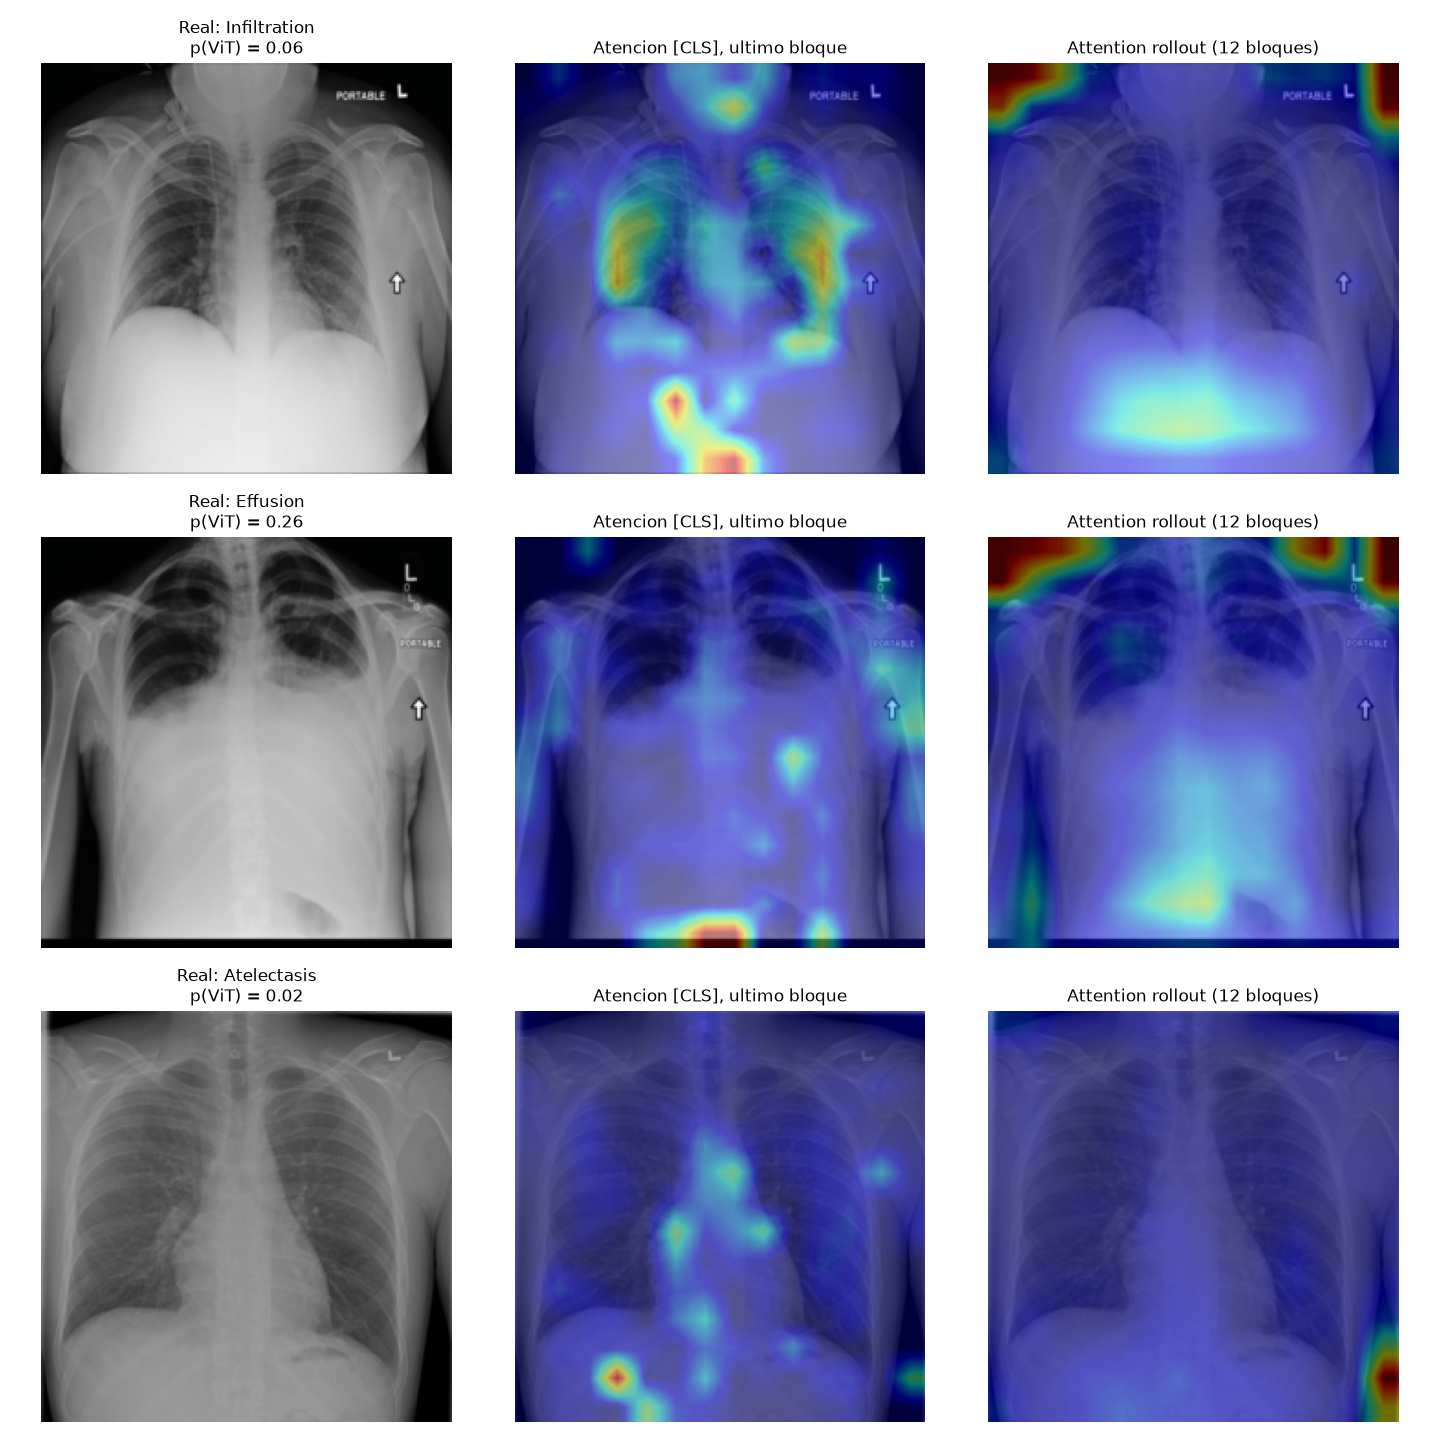
\includegraphics[width=\columnwidth]{attention_example.png}
\caption{ViT-B/16: atención del token \texttt{[CLS]} en el último bloque y \emph{attention rollout} sobre los 12 bloques.}
\label{fig:atencion}
\end{figure}

% =====================================================================
\section{Discusión}
% =====================================================================

\textbf{El Transformer no aporta ventaja en este régimen.} Con 8{,}400 imágenes de entrenamiento, el backbone casi congelado y preentrenamiento en ImageNet-1k, ViT-B/16 no supera a las CNN: su AUROC es estadísticamente indistinguible del de DenseNet121 y ResNet18. Esto es consistente con la observación de que los ViT, al carecer de los sesgos inductivos de las convoluciones, necesitan más datos para superarlas~\cite{dosovitskiy2021vit}, y con estudios previos en radiografía de tórax en los que Transformers y CNN obtienen AUROC muy cercanos~\cite{murphy2022vit} o en los que la ventaja corresponde a diseños híbridos y no a Transformers puros~\cite{yanar2025mamba}. Su curva de validación, sin embargo, es la más estable y su mejor época es la tercera, lo que sugiere que podría beneficiarse más que las CNN de más datos o más épocas.

\textbf{El compromiso desempeño--costo favorece a ResNet18.} El modelo más pequeño en cómputo obtuvo el mejor AUROC, la mayor velocidad de inferencia y la menor memoria. DenseNet121 tiene menos parámetros, pero sus concatenaciones densas lo hacen cuatro veces más lento que ResNet18 en inferencia. ViT-B/16 es el más costoso en todas las métricas sin mejorar el desempeño.

\textbf{La capacidad entrenable explica el sobreajuste.} Aunque el protocolo es idéntico, descongelar el último bloque de cada modelo da 2.2M, 8.4M y 7.1M parámetros entrenables. ResNet18, el de mayor capacidad, aprende más rápido y se sobreajusta desde la época 3; restaurar la mejor época es lo que le permite obtener el mejor resultado. Evaluar en la última época habría penalizado justamente al mejor modelo.

\textbf{La evaluación cambia las conclusiones.} La exactitud por etiqueta es igual a la de un clasificador trivial y el F1 con umbral 0.5 es casi nulo; con estas métricas los tres modelos parecerían inútiles o equivalentes. El AUROC y el F1 con umbral elegido en validación sí permiten compararlos, y los intervalos de confianza muestran que la mayoría de las diferencias observadas no son significativas.

\textbf{La dificultad depende del hallazgo.} Los hallazgos extensos y bien definidos (Emphysema, Edema, Effusion) se detectan mucho mejor que los pequeños (Nodule) o los de definición radiológica ambigua y solapada (Infiltration, Pneumonia), en los tres modelos por igual. Esto sugiere que el límite está más en la resolución y en la calidad de las etiquetas que en la arquitectura. Los valores absolutos son menores que los de CheXNet ($\approx$0.84), que usó el conjunto completo y afinó toda la red.

\textbf{Los mapas de interpretabilidad revelan posibles atajos.} Que los modelos se fijen en marcas de texto o bordes de la imagen en algunos casos es una advertencia práctica: un buen AUROC no garantiza que el modelo use los signos clínicos correctos.

\subsection{Limitaciones}
Se usó un subconjunto aleatorio de 12{,}000 imágenes ($\approx$11\% del conjunto) por restricciones de cómputo y tiempo. Las etiquetas de ChestX-ray14 se extrajeron automáticamente de reportes, por lo que contienen ruido~\cite{oakdenrayner2020exploring}; parte del error medido es ruido de etiqueta y no del modelo. El presupuesto de entrenamiento (cinco épocas y backbone mayormente congelado) impide comparar los valores absolutos con trabajos que afinan la red completa; el objetivo aquí es comparar arquitecturas en igualdad de condiciones. Aunque el protocolo es común, el número de parámetros entrenables difiere entre modelos. Se usó una sola semilla: los intervalos de confianza reflejan la variabilidad del conjunto de prueba, no la del entrenamiento. Las clases raras (Hernia, Pneumonia) tienen muy pocos positivos y pesan igual que las demás en los promedios macro. La reducción a $224\times224$ puede eliminar detalle relevante para hallazgos pequeños, y el volteo horizontal invierte la lateralidad anatómica (por ejemplo, la posición del corazón), lo que podría afectar a hallazgos con lateralidad característica como Cardiomegaly. La ejecución en una GPU AMD con ROCm, sin la implementación de atención eficiente en memoria, hace que el tiempo y la memoria del ViT sean pesimistas frente a una GPU NVIDIA. Finalmente, los ejemplos de interpretabilidad son cualitativos.

% =====================================================================
\section{Conclusiones}
% =====================================================================

Bajo un mismo protocolo y presupuesto, las tres arquitecturas alcanzan un desempeño muy similar en ChestX-ray14 (AUROC promedio de 0.742 a 0.760), y la única diferencia significativa favorece a ResNet18 sobre DenseNet121. ViT-B/16 no mejora a las CNN y es el más costoso: 12 veces más parámetros que DenseNet121 y 13 veces más lento en inferencia que ResNet18. En este escenario, ResNet18 es la opción más eficiente. Metodológicamente, la partición por paciente, la elección de umbrales en validación y los intervalos de confianza fueron decisivos para obtener conclusiones correctas, y los mapas de interpretabilidad muestran que los modelos pueden apoyarse en atajos ajenos a la anatomía.

Como trabajo futuro se propone entrenar con el conjunto completo, afinar la red completa durante más épocas, repetir los experimentos con varias semillas, usar mayor resolución, emplear funciones de pérdida que compensen el desbalance de clases y evaluar cuantitativamente la localización de los mapas de interpretabilidad con las cajas delimitadoras que ChestX-ray14 incluye para un subconjunto de imágenes.

% =====================================================================
\begin{thebibliography}{99}

\bibitem{wang2017chestxray}
X.~Wang, Y.~Peng, L.~Lu, Z.~Lu, M.~Bagheri, and R.~M.~Summers, ``ChestX-ray8: Hospital-scale chest X-ray database and benchmarks on weakly-supervised classification and localization of common thorax diseases,'' in \emph{Proc. IEEE Conf. Computer Vision and Pattern Recognition (CVPR)}, 2017, pp.~2097--2106.

\bibitem{kaggle2018nih}
National Institutes of Health, ``NIH Chest X-rays,'' Kaggle. [Online]. Available: \url{https://www.kaggle.com/datasets/nih-chest-xrays/data}

\bibitem{rajpurkar2017chexnet}
P.~Rajpurkar, J.~Irvin, K.~Zhu, B.~Yang, H.~Mehta, T.~Duan, D.~Ding, A.~Bagul, C.~Langlotz, K.~Shpanskaya, M.~P.~Lungren, and A.~Y.~Ng, ``CheXNet: Radiologist-level pneumonia detection on chest X-rays with deep learning,'' arXiv:1711.05225, 2017.

\bibitem{he2016resnet}
K.~He, X.~Zhang, S.~Ren, and J.~Sun, ``Deep residual learning for image recognition,'' in \emph{Proc. IEEE Conf. Computer Vision and Pattern Recognition (CVPR)}, 2016, pp.~770--778.

\bibitem{huang2017densenet}
G.~Huang, Z.~Liu, L.~van der Maaten, and K.~Q.~Weinberger, ``Densely connected convolutional networks,'' in \emph{Proc. IEEE Conf. Computer Vision and Pattern Recognition (CVPR)}, 2017, pp.~4700--4708.

\bibitem{dosovitskiy2021vit}
A.~Dosovitskiy, L.~Beyer, A.~Kolesnikov, D.~Weissenborn, X.~Zhai, T.~Unterthiner, M.~Dehghani, M.~Minderer, G.~Heigold, S.~Gelly, J.~Uszkoreit, and N.~Houlsby, ``An image is worth 16x16 words: Transformers for image recognition at scale,'' in \emph{Proc. Int. Conf. Learning Representations (ICLR)}, 2021.

\bibitem{vaswani2017attention}
A.~Vaswani, N.~Shazeer, N.~Parmar, J.~Uszkoreit, L.~Jones, A.~N.~Gomez, {\L}.~Kaiser, and I.~Polosukhin, ``Attention is all you need,'' in \emph{Advances in Neural Information Processing Systems (NeurIPS)}, 2017.

\bibitem{deng2009imagenet}
J.~Deng, W.~Dong, R.~Socher, L.-J.~Li, K.~Li, and L.~Fei-Fei, ``ImageNet: A large-scale hierarchical image database,'' in \emph{Proc. IEEE Conf. Computer Vision and Pattern Recognition (CVPR)}, 2009, pp.~248--255.

\bibitem{irvin2019chexpert}
J.~Irvin \emph{et al.}, ``CheXpert: A large chest radiograph dataset with uncertainty labels and expert comparison,'' in \emph{Proc. AAAI Conf. Artificial Intelligence}, 2019.

\bibitem{oakdenrayner2020exploring}
L.~Oakden-Rayner, ``Exploring large-scale public medical image datasets,'' \emph{Academic Radiology}, vol.~27, no.~1, pp.~106--112, 2020.

\bibitem{raghu2021vit}
M.~Raghu, T.~Unterthiner, S.~Kornblith, C.~Zhang, and A.~Dosovitskiy, ``Do vision transformers see like convolutional neural networks?,'' in \emph{Advances in Neural Information Processing Systems (NeurIPS)}, 2021.

\bibitem{murphy2022vit}
Z.~R.~Murphy, K.~Venkatesh, J.~Sulam, and P.~H.~Yi, ``Visual transformers and convolutional neural networks for disease classification on radiographs: A comparison of performance, sample efficiency, and hidden stratification,'' \emph{Radiology: Artificial Intelligence}, vol.~4, no.~6, e220012, 2022.

\bibitem{yanar2025mamba}
E.~Yanar, F.~Kutan, K.~Ayturan, U.~Kutbay, O.~Algın, F.~Hardalaç, and A.~M.~Ağıldere, ``A comparative analysis of the Mamba, Transformer, and CNN architectures for multi-label chest X-ray anomaly detection in the NIH ChestX-ray14 dataset,'' \emph{Diagnostics}, vol.~15, no.~17, 2215, 2025.

\bibitem{selvaraju2017gradcam}
R.~R.~Selvaraju, M.~Cogswell, A.~Das, R.~Vedantam, D.~Parikh, and D.~Batra, ``Grad-CAM: Visual explanations from deep networks via gradient-based localization,'' in \emph{Proc. IEEE Int. Conf. Computer Vision (ICCV)}, 2017, pp.~618--626.

\bibitem{abnar2020rollout}
S.~Abnar and W.~Zuidema, ``Quantifying attention flow in transformers,'' in \emph{Proc. Annual Meeting of the Association for Computational Linguistics (ACL)}, 2020, pp.~4190--4197.

\bibitem{zech2018variable}
J.~R.~Zech, M.~A.~Badgeley, M.~Liu, A.~B.~Costa, J.~J.~Titano, and E.~K.~Oermann, ``Variable generalization performance of a deep learning model to detect pneumonia in chest radiographs: A cross-sectional study,'' \emph{PLoS Medicine}, vol.~15, no.~11, e1002683, 2018.

\bibitem{degrave2021shortcuts}
A.~J.~DeGrave, J.~D.~Janizek, and S.-I.~Lee, ``AI for radiographic COVID-19 detection selects shortcuts over signal,'' \emph{Nature Machine Intelligence}, vol.~3, pp.~610--619, 2021.

\bibitem{kingma2015adam}
D.~P.~Kingma and J.~Ba, ``Adam: A method for stochastic optimization,'' in \emph{Proc. Int. Conf. Learning Representations (ICLR)}, 2015.

\bibitem{paszke2019pytorch}
A.~Paszke \emph{et al.}, ``PyTorch: An imperative style, high-performance deep learning library,'' in \emph{Advances in Neural Information Processing Systems (NeurIPS)}, 2019.

\bibitem{efron1993bootstrap}
B.~Efron and R.~J.~Tibshirani, \emph{An Introduction to the Bootstrap}. New York, NY, USA: Chapman \& Hall, 1993.

\end{thebibliography}

\end{document}
